\section{Results and Discussion}
\label{Results and discussion}
% \setcounter{equation}{0}

\subsection{Introduction to Results and Discussion}

In this section we first assess the model accuracy of our predictive ML models, using metrics as described in \autoref{Methodology}, and summarised in \autoref{tab:methodology-performance-metrics}. This seeks to answer the first research question (1) "To what degree can machine learning algorithms predict the index composition of OSEBX in the next period?". Next, we simulate portfolios in an active trading strategy, where we trade on the predicted additions and deletions made by the ML models. We do so by running a portfolio simulation from 2006 to 2023 and assessing the performance with financial metrics introduced in \autoref{Theoretical background}. This seeks to answer the second research question (2) "To what degree can trading on predicted additions and deletions outperform OSEBX in an active trading portfolio?". Lastly, we repeat the portfolio simulation, but this time in an enhanced index strategy, seeking to answer research question (3) "To what degree can trading on predicted additions and deletions outperform OSEBX in an enhanced index portfolio?"

\subsubsection{Preliminary Machine Learning Models Summary}

We apply logistic regression using GLM, and tree boosting using XGBoost. In XGBoost we use a standard benchmark model (XGBoost benchmark). We also use an XGBoost model with conditional PPT (XGBoost custom). For each index rebalancing event, we predict either 30, 60, or 100 days prior to ED, all of which happens \textit{before} AD. This is indicated in the suffix of the model names, as summarised in \autoref{tab:machine-learning-model-names}. In total, we are analysing nine unique models. All hyperparameters used in the XGBoost-models are summaries in \autoref{xgb-hyperparameters}. 



\begin{table}[H]
\centering
\footnotesize
\begin{tabularx}{\textwidth}{lXXX}
\hline
Model                    & ED-30     & ED-60     & ED-100 \\
\hline
GLM                     & GLM30     & GLM60     & GLM100 \\
XGBoost Benchmark       & XGBB30    & XGBB60    & XGBB100 \\
XGBoost Custom          & XGBC30    & XGBC60    & XGBC100 \\
\hline
\end{tabularx}
\vspace{1em}
\caption{{ML Model Names}}
\subcaption*{Overview of ML-models used. We predict using logistic regression (GLM), XGBoost benchmark (XGBB) and XGBoost with conditional PPT (XGBC). For each of these models, we predict 30, 60, and 100 days before ED, which correspond to the model names.}
\label{tab:machine-learning-model-names}
\end{table}

\subsubsection{Posterior Probability Threshold Applied}

To determine which PPT to apply, we experimented with different thresholds on the models to better understand the direction of the accuracy when changing the threshold. The models seem to be pruned towards predicting more FP and TP classifications compared to FN and TN. Our models are able to correctly predict more additions than deletions, which according to \autoref{fig:index-effect-osebx} might be sub-optimal. \autoref{fig:index-effect-osebx} illustrate that taking short positions on deletions might have higher expected returns than taking long positions on additions. Therefore, we tweaked the PPT slightly upwards. This gave us higher overall accuracy and a more evenly distributed allocation between additions and deletions. In \autoref{tab:glm_accuracy} we show the tweaking of PPT compared to the predictive accuracy for the model GLM30. Here, we choose to illustrate PPT for GLM30, but in general, the other models show a similar pattern as shown for the GLM30 model. 
\vspace{2em}
\begin{table}[H]
\centering
\begin{tabular}{llllllll}
  \hline
Threshold & 0.3 & 0.4 & 0.5 & 0.6 & 0.7 & 0.8& 0.9  \\
\midrule
Accuracy & 0.9394 & 0.9464 & 0.9471 & 0.9482 & 0.9452 & 0.9407 & 0.9149\\
   \hline
\end{tabular}
\vspace{1em}
\caption{{Tuning PPT for ML models}}
\subcaption*{This illustrates the accuracy in relation to PPT for the GLM30 model. We find this model to be somewhat representative, and choose to set PPT for all models to 0.6.}
\label{tab:glm_accuracy}
\end{table}

We therefore continue using 0.6 as our initial PPT in the models, but we are yet to determine the $\varepsilon$ parameter to be applied in XGBoost custom models (where we use the conditional PPT). To understand how the number of predicted changes behave when changing the $\varepsilon$ parameter, we illustrated this relationship in \autoref{fig:beta_plot}, fitted to an XGBoost model making predictions 30 days in advance ED. We point out that the total number of predicted changes is the sum of all predicted changes from 2010 and onward.

\begin{figure}[H]
    \centering
    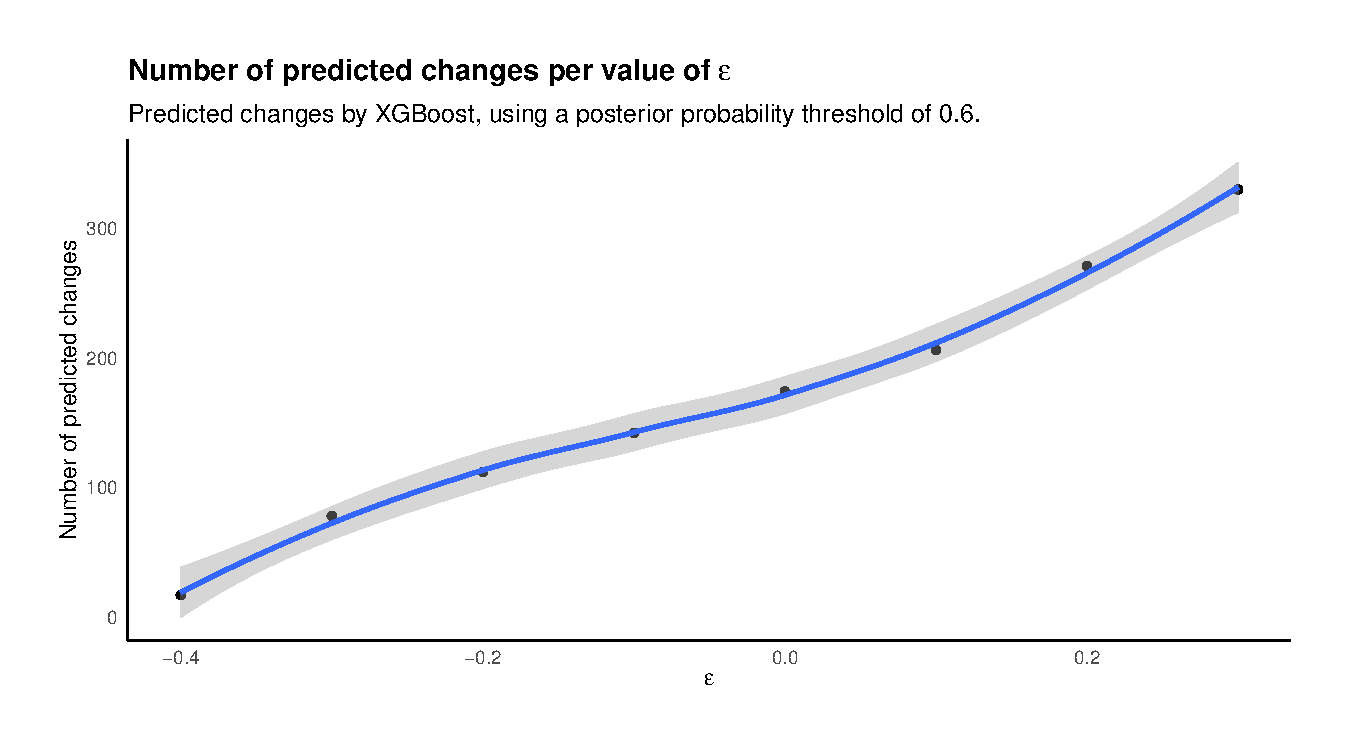
\includegraphics[width=1\textwidth]{images/beta_plot.pdf}
    \caption{{Number of Predicted Changes for Values of $\varepsilon$}}
    \subcaption*{Sum of predicted additions and deletions as a function of $\varepsilon$ in the interval -0.4 to 0.3. Higher $\varepsilon$ correspond to increasing the total number of predicted changes. $\varepsilon$ represents the parameter added or subtracted from the initial PPT, which is fitted to 0.6. In this plot we used an XGBoost model, predicting 30 days ahead of ED.}
    \label{fig:beta_plot}
\end{figure}

\autoref{fig:beta_plot} shows the interval of $\varepsilon$ between -0.4 and 0.3. If we had gone with an even smaller $\varepsilon$, to say -0.6, we would not have gotten any predictions at all. Vice versa, if we had used a $\varepsilon$ of 0.4, we would have gotten $\approx$ 2000 predicted changes. We discarded those cases from the plot to make it easier to read, and because they are irrelevant to our application. 

To decide which $\varepsilon$ to use going forward, we considered different aspects. First of all, we point out that our latter two research questions seek to find out to what degree we can exploit the index effect. The idea of using a conditional PPT is to lower the systematic financial risk and increase the likelihood of buying/selling companies that will be included/excluded from OSEBX. Therefore, we are interested in using a $\varepsilon$ that is higher than 0, because ultimately, we want to increase the number of trades. When $\varepsilon$ is 0, we get the same predictions for XGBoost custom as the XGBoost benchmark model gives, which is a total of about 170 changes. By increasing $\varepsilon$ to 0.2 we predict $\approx$ 270 changes, meaning that the portfolios will be significantly more diversified and eliminating more systematic risk than the portfolios using XGB benchmark and GLM. As we would still like to keep accuracy at an acceptable level compared to the other models, we do not aim to extend the $\varepsilon$ too far and proceed using 0.2 as our $\varepsilon$ parameter in the custom XGBoost models. We would also like to point out that we could have implemented a similar conditional PPT for the GLM models, but we decided to proceed by applying it to the XGBoost models only because they initially are more pruned towards predicting changes than GLM. In practice, the GLM models would require much higher values of $\varepsilon$, and it proved to be more difficult to fit. To conclude this discussion, we proceed using 0.6 as our initial PPT for GLM and XGBB models, and 0.6 $+$/$-$ 0.2 as the conditional PPT for XGBC models.

% RESEARCH QUESTION 1 %%%%%%%%%%%%%%%%%%%%%%%%%%%%%%%%%%%%%%%%%%%%%%%%%%%

\subsection{Research Question (1): To what degree can machine learning algorithms predict the index composition of OSEBX in the next period?}

\subsubsection{Model Accuracy}

In \autoref{confusion_matrix_result} we have illustrated the confusion matrices for the classifications for each model in \autoref{tab:machine-learning-model-names}. 
\begin{table}[H]
\centering
\begin{tabular}{lcccc}
& & GLM & XGBB & XGBC \\
\vspace{1em}
&30 & $\begin{bmatrix} 2729   & 117 \\ 112  & 1462 \end{bmatrix}$ & 
    $\begin{bmatrix} 2683     &  108 \\ 158  &  1471 \end{bmatrix}$ & 
    $\begin{bmatrix} 2639     & 125  \\ 202    &  1454 \end{bmatrix}$\\
\vspace{1em}
$\begin{bmatrix} TN   & FN  \\ FP   &  TP \end{bmatrix}$ & 60 & $\begin{bmatrix} 2711   & 111  \\ 110   &  1458 \end{bmatrix}$ & 
    $\begin{bmatrix} 2666      & 105  \\ 155  &  1464 \end{bmatrix}$ & 
    $\begin{bmatrix} 2628       &  107 \\ 193    & 1462  \end{bmatrix}$  \\
\vspace{1em}
&100 & $\begin{bmatrix} 2698     &  111 \\ 105    &1457  \end{bmatrix}$ & 
     $\begin{bmatrix} 2646   & 114 \\157    & 1454  \end{bmatrix}$ & 
     $\begin{bmatrix} 2605     & 123 \\ 198    &1445  \end{bmatrix}$ \\

\end{tabular}
\vspace{1em}
\caption{{Confusion matrices for all models}}
\subcaption*{The figure shows the confusion matrices for the different models. TN = true negative (we predicted the company not be included on OSEBX, and it did not), FN = false negative (we predicted the company not be included on OSEBX, but it did) FP = false positive (we predicted the company to be included on OSEBX, but it did not) and TP = true positive (we predicted the company to be included on OSEBX, and it did). The matrices show the sum of all rebalancing events since 2010.}
\label{confusion_matrix_result}
\end{table}

First of all, we notice that the models are predicting more TNs than TPs. This is of course as expected, as only 50-80 of the $\approx$ 200 companies on OSEAX are also included on OSEBX. More interestingly, we observe quite evenly matched allocations between FP and FN classifications for the GLM models, meaning that those models are relatively equal in falsely predicting \texttt{index\_cp} = 1 and falsely predicting \texttt{index\_cp} = 0. For the XGBoost models, there are still some imbalances when it comes to allocation between FP and FN, meaning that XGBoost-models are pruned towards predicting more falsely \texttt{index\_cp} = 1 than \texttt{index\_cp} = 0. This can mean that an even higher PPT would even those out, but as our tuning of the PPT showed, that can ultimately decrease overall accuracy. Further, the statistics from the confusion matrices are shown in \autoref{table:accuracy-precision-sensitivity-specificity-f-score}.

\begin{table}[ht]
\centering
\begin{tabular}{llllllll}
  \toprule
Model & Accuracy & Precision & Sensitivity & Specificity & F-score & AUROC & n \\ 
  \midrule
index\_lag1 & 0.9507 & 0.9208 & 0.9399 & 0.9565 & 0.9303  & 0.9446 & 0 \\
  \midrule
GLM100 & 0.9506 & 0.9292 & 0.9328 & 0.9605 & 0.9310 & 0.9789 &    63 \\ 
GLM60 & 0.9497 & 0.9293 & 0.9298 & 0.9607 & 0.9296 & 0.9808 &    76 \\ 
GLM30 & 0.9482 & 0.9259 & 0.9288 & 0.9589 & 0.9274 & 0.9797 &    93 \\ 
XGBB60 & 0.9408 & 0.9331 & 0.9043 & 0.9621 & 0.9184 & 0.9817 &   165 \\ 
XGBB30 & 0.9398 & 0.9316 & 0.9030 & 0.9613 & 0.9171 & 0.9812 &   174 \\ 
XGBB100 & 0.9380 & 0.9273 & 0.9025 & 0.9587 & 0.9148 & 0.9789 &   168 \\ 
XGBC60 & 0.9317 & 0.9318 & 0.8834 & 0.9609 & 0.9069 & 0.9817 &   247 \\ 
XGBC100 & 0.9266 & 0.9216 & 0.8795 & 0.9549 & 0.9000 & 0.9789 &   242 \\ 
 XGBC30 & 0.9260 & 0.9208 & 0.8780 & 0.9548 & 0.8989 & 0.9812 &   271 \\ 
   \bottomrule
\end{tabular}
\vspace{1em}
\caption{{Model Accuracy}}
\subcaption*{Model name, accuracy, precision, sensitivity, F-score, AUROC, and the number of predicted changes to index composition (n). The model index\_lag1 is used as a benchmark model, where the prediction is equal to \texttt{index\_lag1}.}. 
\label{table:accuracy-precision-sensitivity-specificity-f-score}
\end{table}

% tabellen over er oppdatert 08.12.2023

\autoref{table:accuracy-precision-sensitivity-specificity-f-score} show the accuracy, precision, sensitivity, specificity, F-score, AUROC, and the number of predicted changes. In addition, we show a simple model named index\_lag1, where the prediction for the target variable \texttt{index\_cp} is equal to \texttt{index\_lag1}. On accuracy, we notice that the ML models were not able to outperform the simple model. This suggests that \texttt{index\_lag1} is a highly important variable when it comes to predicting index composition. Interestingly, the GLM models were able to outperform the XGBB in terms of accuracy, but we notice that the XGBB and XGBC models generally yield higher AUROC. 

Another interesting observation is that GLM100 has higher accuracy than both GLM60 and GLM30, which seems surprising given that GLM100 makes predictions several months ahead of the rebalancing. One possible explanation is that GLM100 predicts so far ahead of the next rebalancing that the date of prediction is closer to the previous rebalancing than the next. One could therefore possibly expect GLM100 to predict the previous rebalancing with higher accuracy than the upcoming, which in turn can yield almost the same results as the \texttt{index\_lag1} variable, which seems to be severely important when predicting upcoming composition.

Furthermore, we point out that the number of predicted additions and deletions is higher for XGBoost models compared to GLM, with XGBC30 predicting the highest number of changes. A higher number of trades should in turn lower the financial systematic risk. A \textit{significant insight} from assessing model accuracy is that accuracy seems to diminish with a higher number of predicted changes. To further illustrate this point: the simple model (index\_lag1) has better accuracy than any of the other nine models but does not predict any changes to the index composition. When trying to exploit the index effect, such a model would therefore not be viable, and we must accept lower accuracy if we want to exploit the index effect.

\subsubsection{AUROC}

\begin{figure}[H]
    \centering
    \footnotesize
    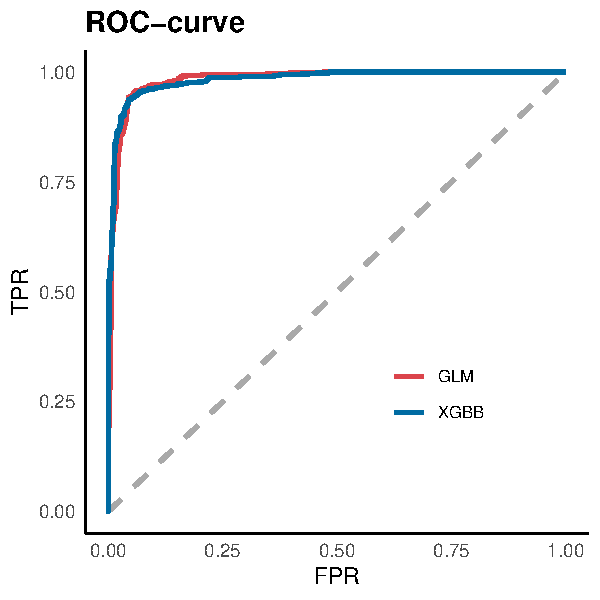
\includegraphics[width=0.5\linewidth]{images/roc_curve.pdf}
    \caption{{ROC Curve for 30-day predictions}}
    \subcaption*{Receiver operating characteristic (ROC) curve illustrated for the GLM30 and XGBB30 ML models. Area Under ROC is 0.9797 and 0.9812 for the GLM30 and XGBB30 respectively. }
    \label{fig:roc-curve-for-models}
\end{figure}

 \autoref{fig:roc-curve-for-models} show the ROC curve for models GLM and XGBB, for the 30-day prediction horizon. Compared to \autoref{fig:area-under-roc-curve-illustration}, the characteristics from the ROC-curve in \autoref{fig:roc-curve-for-models} seem to further support the models' overall ability to predict index-composition, supporting the findings from \autoref{table:accuracy-precision-sensitivity-specificity-f-score}. Notice that we did not include the XGBC models in this plot, because the plot is generated by using the estimated likelihoods from the models, which is the same for both XGBB and XGBC models.
 
\subsubsection{Accuracy over Time}

Furthermore, we illustrate the models' performance over time, as we are dealing with a time series. \autoref{fig:machine-learning-results} show the ML model's accuracy over time, completed with the number of changes (additions and deletions) predicted for each period, and the number of true changes captured. As expected from \autoref{table:accuracy-precision-sensitivity-specificity-f-score}, GLM and XGBB models seem to yield better accuracy for most periods, while predicting fewer changes than XGBC. Once again our results suggest a negative relationship between accuracy and the number of predicted changes. 

\begin{figure}[H]
    \centering
    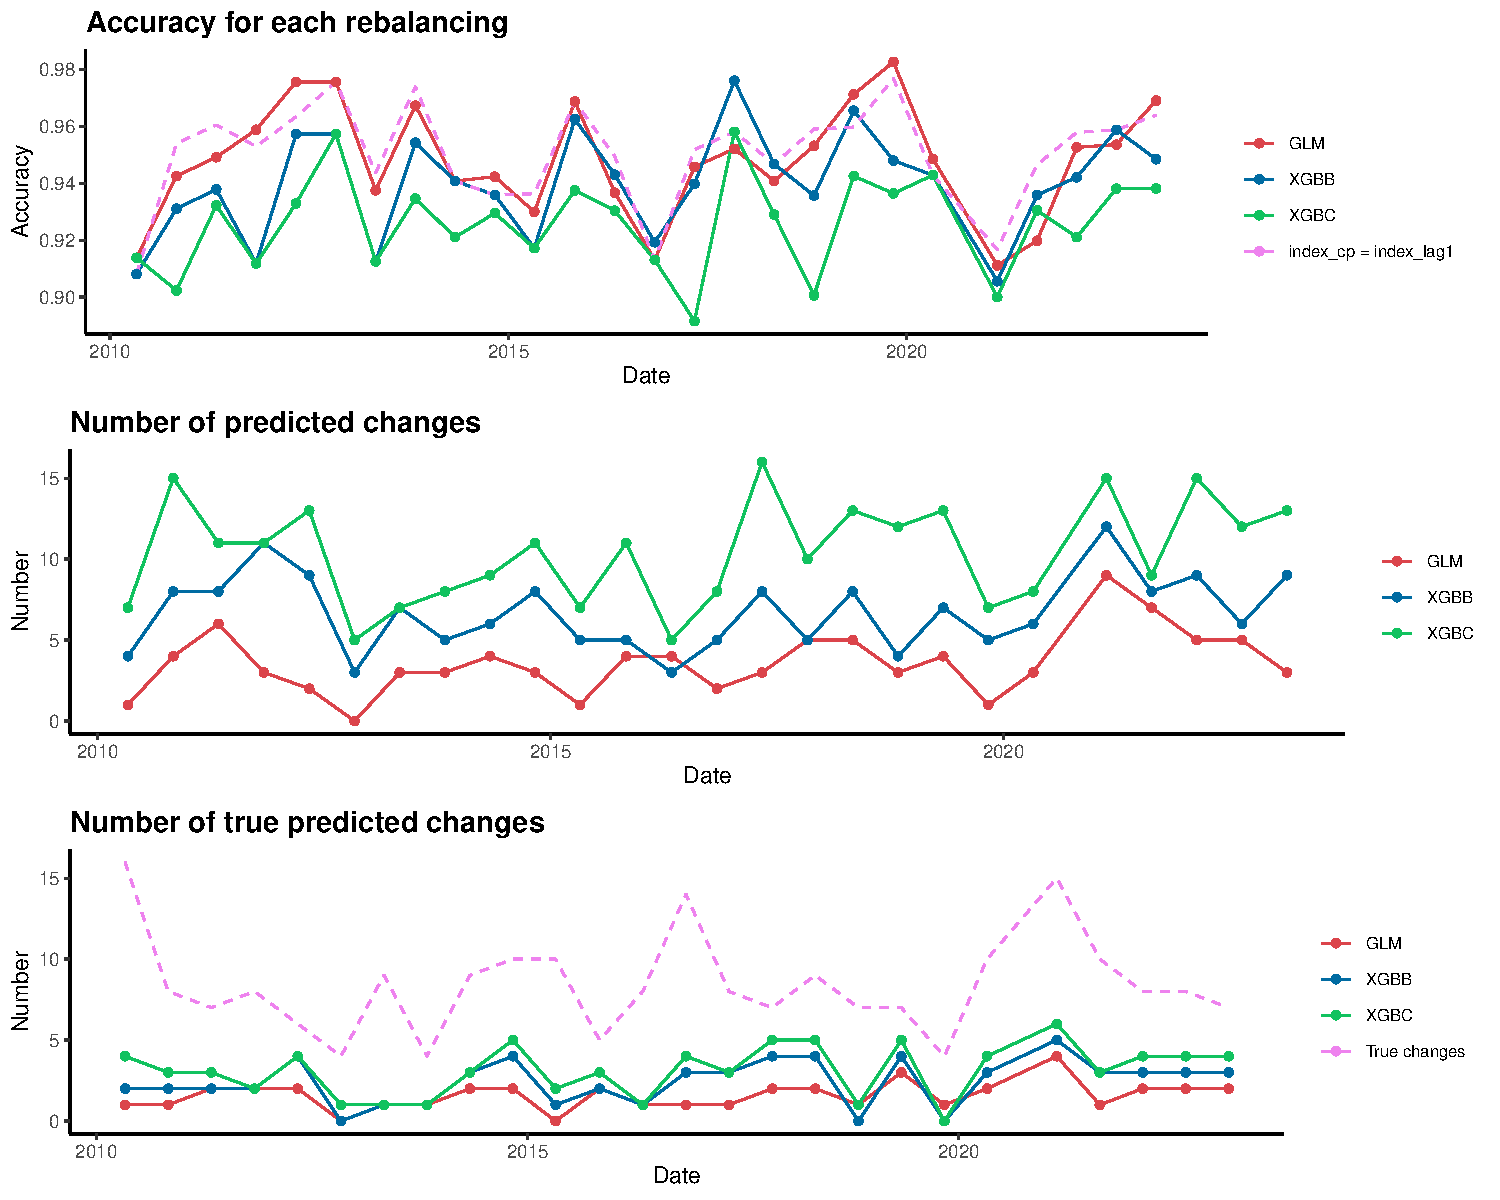
\includegraphics[width=\textwidth]{images/machinelearning_res.pdf}
    \caption{{ML Results over time, 30-day prediction horizon}}
    \subcaption*{Illustrations of how the models GLM30, XGBB30, and XGBC30 perform over the course of the period from 2010 to 2023. Please note that the simple model (index\_lag1) is illustrated in the accuracy plot. }
    \label{fig:machine-learning-results}
\end{figure}

Another insight from \autoref{fig:machine-learning-results} is that we are nowhere near capturing all true changes. As mentioned earlier, if we had bought all companies outside of OSEBX and sold all companies at OSEBX, we would have captured all the changes. However, that would significantly dilute the index effect, and we therefore need to keep accuracy at a reasonable level even for the XGBC models. From these results, we do however learn that the XGBC models are able to capture more of the true changes than the GLM and XGBB models.

\subsubsection{Variable Importance Plot}
We do already understand that the \texttt{index\_lag1} variable is important when predicting index composition, but we have yet to explore the importance of the remainder of the variables. \autoref{fig:variable-importance-plot-result} show variable importance for our GLM- and XGBoost models predicting 30 days prior to ED respectively.

\begin{figure}[H]
    \centering
    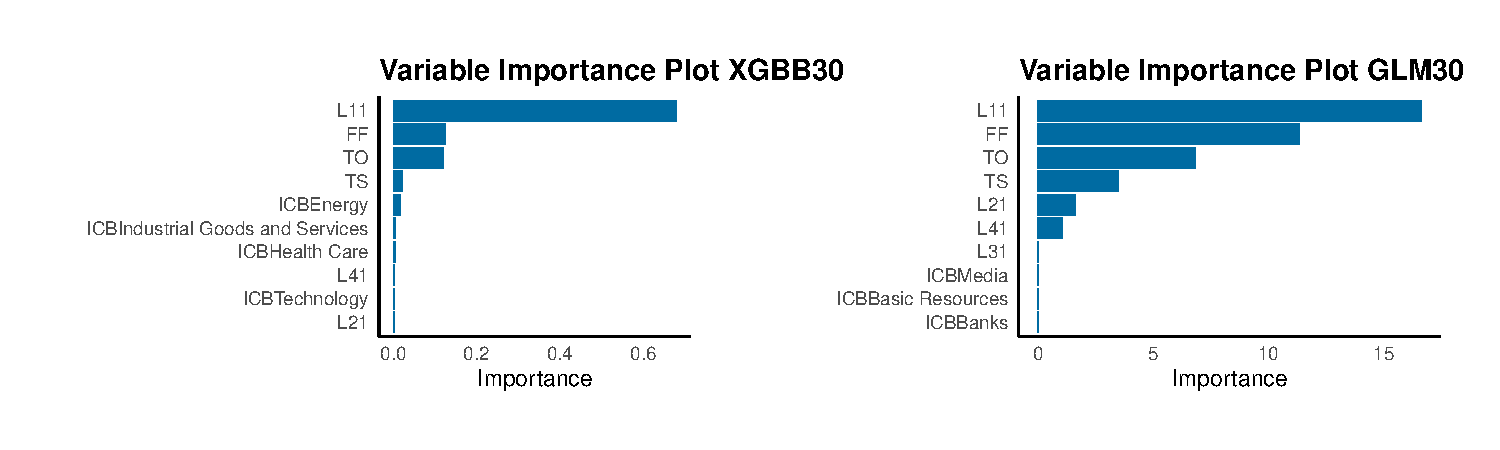
\includegraphics[width=\textwidth]{images/vip.pdf}
    \caption{{VIP for XGBB30 and GLM30}}
    \subcaption*{Please see \autoref{tab:final-data-set-predictor-target} for explanation for all variable abbreviations. Notice that the x-axis measurement differs between the two plots and each plot must be read independently.}
    \label{fig:variable-importance-plot-result}
\end{figure}

 For GLM and XGBB, the variable \texttt{index\_lag1} proves to be the most important one, followed by \texttt{free\_float}, \texttt{turnover\_eob}, and \texttt{trading\_status}. Understanding why \texttt{index\_lag1} is most important, we remember that most of the 50-80 companies on OSEBX stay from one period to the next. This includes large Norwegian companies, such as Equinor and Telenor. Therefore, predicting large and liquid companies staying on OSEBX from one period to the next is quite easy, with similar intuition for small listed companies staying off OSEBX. The \texttt{index\_lag1} variable is however not suited for explaining the cases where the model predicts a change in the response variable compared to the previous period. This must then be explained by the other variables, seemingly by \texttt{free\_float}, \texttt{turnover\_eob}, and \texttt{trading\_status}, which are the variables taken directly out of the OSEBX rule book. Furthermore, the two models differentiate when it comes to the 5th, 6th, and 7th most important variables. The GLM model seems to depend more on the other lag variables, whereas the XGBoost models are more dependent on the \texttt{icb\_supersector} variables. 


\subsubsection{Conclusion for Research Question (1)}

In our first research question, we ask "To what degree can ML predict index composition in the next period?". In this section, we have discussed the models' overall performance. The simple model which only predicts using \texttt{index\_lag1}, gave the highest accuracy (0.9507), but GLM100 followed closely with an accuracy of 0.9506. This means that we were able to predict more than 95\% of all observations correctly, and we conclude that ML algorithms can predict the upcoming index composition on OSEBX with high accuracy. Furthermore, we have in this section learned that there might exist a trade-off between model accuracy and the total number of predicted changes made by the ML algorithms. This finding is a \textit{central} insight in our thesis. This can cause great consequences in the following section where we simulate portfolios based on the predicted additions and deletions obtained by the models. 

% RESEARCH QUESTION 2 %%%%%%%%%%%%%%%%%%%%%%%%%%%%%%%%%%%%%%%%%%%%%%%%%%%

\subsection{Research Question (2): To what degree can trading on predicted additions and deletions outperform OSEBX in an active trading portfolio?}

In the previous section, we investigated the model accuracy of GLM and XGBoost. In this section, we simulate a portfolio in the period from 2010 to 2023, where we trade on the predicted additions and deletions made by our models. In the portfolio simulation, we consider the number of rebalancing events to predict. We have considered the data available, and find it is suitable for the first rebalancing period to start in 2010. In other words, the first train data set is from 2006 until the first test period in May of 2010. The portfolio simulation ended after the last rebalancing event of March 2023. 

\subsubsection{Active Trading Strategy}

Our trading strategy can be summarised as the following: we buy the companies that the ML models predict to enter OSEBX, and we sell the companies that the ML models predict to exit. The additions/deletions are bought/sold on the date of prediction, and sold/bought at ED. This has several implications. First, we are only allowed to buy companies that are not included in the index at the time of prediction, and we are only allowed to sell companies that currently are on the index. Second, it requires us to expand the strategy to manage the portfolios outside of the active trading period (outside the trading window between prediction and ED). As we want to beat OSEBX, we have decided to take a long position in OSEBX when outside of the trading window. This means that any potential excess returns must come from the active trading period. Thirdly, an important implication is that by using this strategy, we will \textit{never} trade against the index effect in the active period. This is because we are not allowed to buy companies exiting, and not allowed to sell companies entering. 


In a long position, one expects the stock price to rise, and in a short position, one expects the stock price to fall \parencite{jacobs-long-short}. Looking at the index effect in \autoref{fig:index-effect-osebx}, we would like to capture both the rising stock prices by going long on additions and falling stock prices by going short on deletions. In practice, this includes finding combinations where \texttt{index\_lag1=0} is paired with the predicted \texttt{index\_cp=1} (addition, we take a long position), or where \texttt{index\_lag1=1} is paired with the predicted \texttt{index\_cp=0} (deletion, we take a short position). In practice, we simulate two implementations of our strategy. The first strategy includes going long-short, meaning that we are allowed to go both long and short. On the contrary, our second strategy uses long-only positions. The portfolios we simulate and analyse can be summaries as in \autoref{tab:portfolio-names}. 

\begin{table}[H]
\centering
\footnotesize
\begin{tabularx}{\textwidth}{llXXX}
\hline
Model          & Strategy         & ED-30     & ED-60     & ED-100 \\
\hline
GLM           &   Long-short     & GLM30     & GLM60     & GLM100 \\
XGBoost Benchmark&  Long-short      & XGBB30    & XGBB60    & XGBB100 \\
XGBoost Custom  &  Long-short       & XGBC30    & XGBC60    & XGBC100 \\
\midrule
GLM            &   Long-only       & GLM30L     & GLM60L     & GLM100L \\
XGBoost Benchmark &  Long-only     & XGBB30L    & XGBB60L    & XGBB100L \\
XGBoost Custom    &   Long-only    & XGBC30L    & XGBC60L    & XGBC100L \\
\hline
\end{tabularx}
\vspace{1em}
\caption{{Simulated Portfolio Names}}
\subcaption*{Overview of the portfolio names. Notice that the portfolios trade on predicted changes made by the corresponding model from \autoref{tab:machine-learning-model-names}.  The long-short portfolios trade using both predicted additions and deletions. The long-only portfolios trade using only the predicted additions. Long-only portfolios are denoted by the suffix L at the end of the name. }
\label{tab:portfolio-names}
\end{table}

As mentioned in \autoref{introduction}, Euronext rebalances OSEBX twice each year, which is done on ED. Since 2020, ED has been the third Friday of March and September, and before 2020, ED was the first trading day of June and December. Depending on the prediction horizon of 30, 60, or 100 days prior to ED, the active portfolio will be significantly shorter than a year. \autoref{fig:timeline-investment-horizon} illustrates the timeline of the active trading portfolio investment horizon. 

\begin{figure}[H]
    \centering
    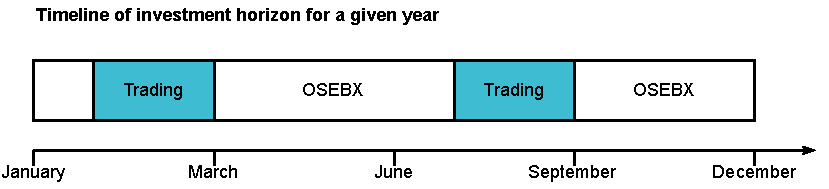
\includegraphics[width=\linewidth]{images/investment-horizon.drawio.pdf}
    \vspace{1em}
    \caption{{Timeline of Investment Horizon}}
    \subcaption*{During the year, our portfolios can be in two states. (1) in an active trading period, between the prediction and the ED. (2) in a passive period, meaning that the money is invested in OSEBX.}
    \label{fig:timeline-investment-horizon}
\end{figure}

\subsubsection{Financial Assumptions}
Next, we discuss the underlying financial assumptions of our portfolio simulation. These are important to make the results robust and practically applicable. The assumptions can be summarised as (1) transaction costs, (2) liquidity, (3) portfolio weights, and (4) interest rate on short positions.

Transaction costs include the brokerage fees when completing a trade \parencite{coase-transaction-costs}. This can come from either brokers implementing the trade by finding a counterpart directly or using a highly advanced trading algorithm supplied by a broker. Electronic trading algorithms typically have lower transaction costs and can utilise strategies, such as completing trades using VWAP. In the portfolio simulation, we take into account the transaction cost by subtracting a cost per trade made. We use basis points (bps) when discussing trading cost, where 1 bps is equal to 0.01\%. \textcite{nbim-investing-in-equities} report commission rates between 5$-$10 bps during the last two decades, with about 2 bps for electronic trades. \textcite{dnb-transaction-costs} list a fee of 4 bps per transaction for large private investors. In the portfolio simulation, we do electronic trades using VWAP, and assuming we can trade on the terms for large investors according to \textcite{dnb-transaction-costs}, we assume a transaction cost of 4 bps. 

Liquidity refers to the availability to which stocks can be traded without significantly altering their prices \parencite{hicks-liquidity}. In practice, stocks on OSEBX may not be available to trade at every given point in time. Still, we conclude that assuming full liquidity for our stocks can be justified. We will be trading stocks on OSEBX that either are on the index or are likely to be on it for the next period. Stocks of these types will have the characteristics of high \texttt{trading\_status}, representing high liquidity. Using this assumption, we say that all stocks are available, and trades are done using VWAP. 

For predicted trades made by the ML model, we must determine the weighting of each security in our active trading portfolio \parencite{frost-portfolio-weights}. We considered different approaches, either to (1) give stocks weights based on the estimated likelihood from the ML model, or to (2) give stocks equal weights. In a practical setting one could argue that weighting smaller or larger positions based on the statistical likelihood is an effective approach, although we decide to weight the positions equally. In short, this is due to ease of implementation, and a lack of an effective converter from probability to weight. 

When taking short positions, one has to borrow a number of stocks from a third party \parencite{jacobs-long-short}. This comes with an interest rate cost, as the original stock owner is compensated for giving up the opportunity to trade during the lending period. The short-position interest rate depends on a variety of factors, including supply of short-sellers. \textcite{nordnet-short-interest-rate} state a short-position interest rate of 4\% annually, and this is what we use in our simulations. Furthermore, regarding short positions, we have used a maximum limit of what the short position might rise to before we are forced to buy back the position. This limit is 100 \%, meaning that if the stock price doubles in value, then we are forced to buy it back and we will get a return of -100\%. In other words, this diminishes the loss, to the maximum loss in a long position.

To sum up, our financial assumptions aim to be conservative, but yet insight-full as shown in \autoref{tab:trading-financial-assumptions}. This is to increase the robustness of our findings and make them valid in a practical setting. 

\begin{table}[H]
\centering
\begin{tabular}{ll}
\hline
Financial & Assumption \\
\hline
Transaction cost trades   & 4 bps   \\ 
Transaction cost OSEBX  & 4 bps \\
Liquidity   & Full \\ 
Price  & VWAP \\ 
Stock weights in portfolio  & Equal \\ 
Risk-free rate $R_f$ & $\approx$ 1.46\% annually \\
Short-position interest rate & 4\% annually \\
\hline
\end{tabular}
\vspace{1em}
\caption{{Summary of Financial Assumptions in the Trading Portfolios}}
\subcaption*{These assumptions lay the basis for our simulations. They aim to be as accurate in a practical sense as possible. }
\label{tab:trading-financial-assumptions}
\end{table}

\subsubsection{Application of the Portfolio Simulations}

 Before presenting portfolio performance, we present a brief explanation to how the simulations are executed. First, the ML models generate a set of predictions, for 30-, 60-, and 100-days in advance of the ED. The data frame in which the predictions are stored is then filtered, so that only the cases where the prediction is different from the classification in the previous period are left. Next, the VWAP is extracted for each recommended trade on both ED and on the date of prediction, depending on the prediction horizon. The return of the position is then determined as shown in \autoref{return_explaination}, where $r_l$ is return on long-positions, and $r_s$ is return on short-positions, $p_0$ is the VWAP of the stock at the start of the trading period, and $p_1$ is the VWAP at the end. 

\begin{equation}
\begin{aligned}
    r_l = \frac{p_1 - p_0 }{p_0} &  ,  &r_s = \frac{p_0 - p_1 }{p_0} 
    
\label{return_explaination}
\end{aligned}
\end{equation}
Next, we take the average of each return per trading period (because we assume equal weighting in our portfolios), and use this return as the period return. This operation is done for each trading period, and we are left with the portfolio development over time. The amount of money that is held at the beginning of the trading period is then multiplied by the average growth factor (the average return plus 1). The same logic applies to the passive periods, where the money is invested in OSEBX. Transaction costs are applied at the start and end of each trading period, and the short interest rate is subtracted from the calculated return on any short position. This is explained in greater detail in \autoref{APPENDIX Portfolio Simulation Algorithm}. In \autoref{APPENDIX Portfolio Simulation of GLM100-portfolio} we also show an example of a simulated portfolio, namely the GLM100 portfolio.

\subsubsection{Performance in a Capital Asset Pricing Model}

 The financial metrics for our respective active trading portfolios are shown in \autoref{tab:new-performance-trading-return-sigma-sharpe-alpha-beta-te-ir}, sorted by decreasing SR. The results in \autoref{tab:new-performance-trading-return-sigma-sharpe-alpha-beta-te-ir} can be compared to the desired metrics in \autoref{tab:metrics-ranges-implications}. All calculations are done using monthly returns, except TE$_{ann}$. Notice that the names of portfolios in \autoref{tab:new-performance-trading-return-sigma-sharpe-alpha-beta-te-ir} correspond to the ML model used to generate trade predictions, as shown in \autoref{tab:portfolio-names}. 

\begin{table}[H]
\centering
\footnotesize
\begin{tabularx}{\textwidth}{Xllllllll}
\toprule
Portfolio & $R_p-R_b$ & $R_p$ & $\sigma_p$ & SR & $\alpha$_{CAPM} & $\beta$ & TE_{ann} & IR \\
\midrule
OSEBX & 0 & 0.0095 & 0.0423 & 0.1981 & 0.0002 & 1.0148 & 0.0000 &  \\ 
\midrule
   GLM60 & 0.0095  & 0.0190 & 0.0756 & 0.2367 & 0.0139 & 0.4966 & 0.2599 & 0.1268 \\ 
   GLM30 & 0.0034  & 0.0129 & 0.0511 & 0.2309 & 0.0048 & 0.8634 & 0.1260 & 0.0940 \\ 
  XGBC30 & 0.0017  & 0.0112 & 0.0441 & 0.2289 & 0.0026 & 0.9249 & 0.0789 & 0.0755 \\ 
  GLM100 & 0.0087  & 0.0182 & 0.0757 & 0.2257 & 0.0133 & 0.4684 & 0.2668 & 0.1132 \\ 
  XGBB30 & 0.0010  & 0.0105 & 0.0488 & 0.1917 & 0.0016 & 0.9536 & 0.1056 & 0.0321 \\  
  XGBC60 & -0.0029 & 0.0066 & 0.0480 & 0.1138 & -0.0004 & 0.7285 & 0.1383 & -0.0731 \\ 
  XGBB60 & -0.0019 & 0.0076 & 0.0608 & 0.1073 & 0.0020 & 0.5532 & 0.2095 & -0.0306 \\ 
 XGBC100 & -0.0038 & 0.0057 & 0.0443 & 0.1027 & 0.0017 & 0.3470 & 0.1782 & -0.0744 \\ 
 XGBB100 & -0.0058 & 0.0037 & 0.0539 & 0.0487 & -0.0012 & 0.4696 & 0.1947 & -0.1024 \\ 
 \midrule
 XGBC30L & 0.0032  & 0.0127 & 0.0482 & 0.2398 & 0.0034 & 1.0065 & 0.0903 & 0.1222 \\ 
 XGBB30L & 0.0033  & 0.0128 & 0.0500 & 0.2335 & 0.0033 & 1.0386 & 0.0990 & 0.1158 \\ 
  GLM30L & 0.0009  & 0.0104 & 0.0460 & 0.2011 & 0.0012 & 0.9942 & 0.0674 & 0.0450 \\ 
 XGBB60L & 0.0011  & 0.0106 & 0.0543 & 0.1751 & 0.0019 & 0.9428 & 0.1361 & 0.0288 \\ 
 XGBC60L & 0.0004  & 0.0099 & 0.0505 & 0.1737 & 0.0008 & 0.9843 & 0.1063 & 0.0131 \\ 
  GLM60L & 0.0002  & 0.0097 & 0.0553 & 0.1550 & 0.0002 & 1.0340 & 0.1187 & 0.0056 \\ 
XGBC100L & 0.0011  & 0.0106 & 0.0649 & 0.1468 & 0.0035 & 0.7391 & 0.2078 & 0.0191 \\
XGBB100L & 0.0015  & 0.0110 & 0.0682 & 0.146 & 0.00324 & 0.826 & 0.211 & 0.0255 \\ 
 GLM100L & -0.0031 & 0.0064 & 0.0669 & 0.0797 & -0.0033 & 1.0614 & 0.1809 & -0.0583 \\ 
\bottomrule
\end{tabularx}
\vspace{1em}
\caption{{CAPM Portfolio Performance for Active Trading Strategies Using Monthly Returns}}
\subcaption*{Risk free interest rate is $\approx$ 0.12 \% per month. The market return is assumed to be the return of OSEAX during the same period, which gave a monthly average return of $\approx$ 0.92\%. Both the risk-free interest rate and the market return are calculated based on (\cite{bernt-fama-french}) in the period from January 31st, 2010 to May 31st, 2022. TE and information ratio is calculated in relation to OSEBX, as this is the index we are aiming to beat. The table is sorted after SR. The analysed period is from January 31st, 2010 to May 31st, 2022. $R_b$ represents the return of the benchmark index OSEBX, so the first column shows excess returns in relation to OSEBX. }
\label{tab:new-performance-trading-return-sigma-sharpe-alpha-beta-te-ir}
\end{table}

Please note that we have defined the market to be OSEAX, as this is the pool of stocks we can buy or sell. Our first observation is that several portfolios yield higher returns $R_p$ than OSEBX. Especially the GLM portfolios yield exceptional returns (GLM60 yielding twice the return of OSEBX). However, those portfolios tend to also be involved with higher risk $\sigma_p$. Taking this into consideration, we observe SR, where the XGBC30L portfolio excels. It is, however, closely followed by the portfolios GLM60, GLM30, XGBC30, GLM100 and XGBB30L. All of these portfolios outperform OSEBX in terms of SR, which seems promising. Furthermore, we observe the biggest alphas $\alpha_{CAPM}$ in GLM60 and GLM100. The high $\alpha_{CAPM}$ for those two portfolios is likely caused by the low correlation with the market ($\beta$) and exceptional returns. At this stage, we would expect this $\alpha_{CAPM}$ to diminish after adjusting for FF3 later on. We also observe notable $\alpha_{CAPM}$ for GLM30, XGBC30, XGBC30L and XGBB30L. Furthermore, the calculated betas $\beta$ seems somewhat surprising, considering the risk $\sigma_p$ involved with several of the portfolios. In general, a risky portfolio is considered to have a high beta (namely, greater than 1). In the long-short portfolios we do however trade on short-positions, which in the active trading periods can constitute a negative correlation with the market, and in turn, lower the beta $\beta$ (being the correlation coefficient with the market). When considering the long-only portfolios we observe somewhat more expected results, with $\beta$ varying from 0.73 to 1.04. In conclusion, several models outperform OSEBX in the world of CAPM, both on $R_p$, $SR$, and $\alpha_{CAPM}$. Further, we investigate the portfolio's exposure to risk.

\subsubsection{Fama-French 3 factor Model on Active Portfolios}

Going further than CAPM portfolio performance, we want to understand if the excess returns can be explained by the risk factors in an FF3 model. We run a linear regression using portfolio returns minus risk-free rate as the dependent variable, and factors SMB, HML, and the market risk premium (see \autoref{Theoretical background}) as independent variables. The FF3 factors introduced in \autoref{Theoretical background} are retrieved from \textcite{bernt-fama-french}, as discussed in \autoref{Data}. 

Note that \textcite{bernt-fama-french} report Fama-French factors for OSE, which is somewhat different from OSEBX. Because OSEAX represents more of the companies on OSE than OSEBX does, we argue that the risk factors are representing OSEAX to a higher extent than OSEBX. We therefore use OSEAX as the market in the FF3 regressions. We have also done the same regressions using OSEBX as the market, which is shown in \autoref{ff3-osebx}, to check for any significant differences.


% new updated 14.12.2023
\begin{table}[H] 
\centering 
\footnotesize
\begin{tabularx}{\textwidth}{XXXX|XXX|XXX|l} 
\\[-2ex]\hline 
\hline \\[-2ex] 
 & \multicolumn{10}{c}{\textit{Dependent variable:}} \\ 
\cline{2-11} 
\\[-2ex] 
 & \multicolumn{3}{c}{GLM} & \multicolumn{3}{c}{XGBB} & \multicolumn{3}{c}{XGBC} & \\
 \cline{2-10}
 \\[-2ex] 
 & 30 & 60 & 100 & 30 & 60 & 100 & 30 & 60 & 100 & OSEBX \\ 
 \cline{2-10} \\
 MR & 0.890$^{***}$ & 0.553$^{***}$ & 0.510$^{***}$ & 0.958$^{***}$ & 0.545$^{***}$ & 0.457$^{***}$ & 0.938$^{***}$ & 0.729$^{***}$ & 0.337$^{***}$ & 1.022$^{***}$ \\ 
  & (0.075) & (0.149) & (0.151) & (0.060) & (0.117) & (0.104) & (0.046) & (0.078) & (0.087) & (0.017) \\
   & & & & & & & & & & \\ 
 SMB & $-$0.166$^{**}$ & $-$0.133 & $-$0.129 & $-$0.105$^{*}$ & $-$0.068 & 0.138 & $-$0.124$^{***}$ & $-$0.058 & 0.101 & $-$0.042$^{**}$ \\ 
  & (0.076) & (0.150) & (0.152) & (0.061) & (0.117) & (0.104) & (0.046) & (0.078) & (0.087) & (0.017) \\ 
   & & & & & & & & & & \\ 
 HML & $-$0.055 & $-$0.219$^{**}$ & $-$0.153 & 0.029 & 0.070 & $-$0.005 & $-$0.008 & 0.023 & 0.007 & $-$0.016 \\ 
  & (0.056) & (0.110) & (0.112) & (0.045) & (0.086) & (0.077) & (0.034) & (0.058) & (0.064) & (0.013) \\ 
   & & & & & & & & & & \\ 
 $\alpha$_{FF3} & 0.006$^{**}$ & 0.013$^{**}$ & 0.013$^{**}$ & 0.003 & 0.004 & $-$0.003 & 0.004$^{**}$ & 0.001 & 0.0004 & 0.001 \\ 
  & (0.003) & (0.006) & (0.007) & (0.003) & (0.005) & (0.004) & (0.002) & (0.003) & (0.004) & (0.001) \\ 
   & & & & & & & & & & \\   
\hline \\[-3ex] 
Obs & 148 & 148 & 148 & 148 & 148 & 148 & 148 & 148 & 148 & 148 \\ 
R$^{2}$ & 0.494 & 0.099 & 0.078 & 0.647 & 0.145 & 0.138 & 0.746 & 0.388 & 0.112 & 0.962 \\ 
R$^{2}$_{adj} & 0.484 & 0.080 & 0.059 & 0.639 & 0.127 & 0.120 & 0.740 & 0.375 & 0.093 & 0.961 \\ 
\hline 
\hline \\[-2ex] 
\textit{Note:}  & \multicolumn{10}{r}{$^{*}$p$<$0.1; $^{**}$p$<$0.05; $^{***}$p$<$0.01} \\ 
\end{tabularx}
\vspace{1em}
\caption{{FF3 Regression: Long-Short Active Portfolios}} 
\subcaption*{The table shows the regression summary of the long-short portfolios return net of risk-free interest rate against market risk premium (RM), the small minus big factor (SMB), and the high minus low factor (HML). The market is considered to be OSEAX, the same as we used as the market used in \autoref{tab:new-performance-trading-return-sigma-sharpe-alpha-beta-te-ir}. Notice that the factors are reported for OSE, and was obtained by \textcite{bernt-fama-french}. We, therefore, decided to use OSEAX as the market, as this more closely represents the market that the factors express.
}
\label{fama-french-trading-long-short} 
\end{table} 


In \autoref{fama-french-trading-long-short}, we find statistically significant positive alpha $\alpha_{FF3}$ at a 95\% confidence level for portfolios GLM30, GLM60, GLM100, and XGBC30, all outperforming the benchmark index OSEBX $\alpha_{FF3}$ of 0.001. This indicates that the mentioned portfolios produce excess returns that are not fully explained by FF3. In comparison to the findings in \autoref{tab:new-performance-trading-return-sigma-sharpe-alpha-beta-te-ir}, we see that the GLM60 and GLM100 portfolios diminish in FF3-regression (compared to the $\alpha_{CAPM}$ reported in CAPM), whereas both GLM30 and XGBC30 increases slightly. This can suggest that the GLM30 and XGBC30 have negative exposure to the risk factors. This is further supported by the correlation coefficients for both SMB and HML. There might also be a source of error coming from the difference between what we have defined as the market, OSEAX, and OSE, on which the risk factors are based. 

% 14 december fama french
\begin{table}[H] \centering  
\footnotesize
\begin{tabularx}{\textwidth}{XXXX|XXX|XXX|l} 
\\[-2ex]\hline 
\hline \\[-2ex] 
 & \multicolumn{10}{c}{\textit{Dependent variable:}} \\ 
\cline{2-11} 
\\[-2ex] 
 & \multicolumn{3}{c}{GLML} & \multicolumn{3}{c}{XGBBL} & \multicolumn{3}{c}{XGBCL} & \\
 \cline{2-10}
 \\[-2ex] 
 & 30 & 60 & 100 & 30 & 60 & 100 & 30 & 60 & 100 & OSEBX \\ 
 \cline{2-10} \\
 MR & 1.001$^{***}$ & 1.042$^{***}$ & 1.066$^{***}$ & 1.030$^{***}$ & 0.936$^{***}$ & 0.795$^{***}$ & 1.006$^{***}$ & 0.984$^{***}$ & 0.719$^{***}$ & 1.022$^{***}$ \\ 
  & (0.045) & (0.074) & (0.104) & (0.055) & (0.079) & (0.025) & (0.052) & (0.064) & (0.118) & (0.017) \\ 
   & & & & & & & & & & \\ 
 SMB & $-$0.072 & 0.026 & 0.143 & 0.003 & 0.055 & 0.264 & $-$0.007 & 0.032 & 0.170 & $-$0.042$^{**}$ \\ 
  & (0.045) & (0.074) & (0.105) & (0.055) & (0.080) & (0.025) & (0.053) & (0.064) & (0.119) & (0.017) \\ 
   & & & & & & & & & & \\ 
 HML & 0.001 & $-$0.056 & $-$0.098 & 0.038 & 0.005 & 0.017 & 0.002 & $-$0.020 & 0.024 & $-$0.016 \\ 
  & (0.033) & (0.054) & (0.077) & (0.041) & (0.059) & (0.018) & (0.039) & (0.047) & (0.088) & (0.013) \\ 
   & & & & & & & & & & \\ 
 $\alpha$_{FF3} & 0.002 & $-$0.001 & $-$0.006 & 0.004 & 0.001 & $-$0.001 & 0.004 & 0.0002 & 0.001 & 0.001 \\ 
  & (0.002) & (0.003) & (0.005) & (0.002) & (0.003) & (0.001) & (0.002) & (0.003) & (0.005) & (0.001) \\ 
   & & & & & & & & & & \\ 
\hline \\[-2ex] 
Obs & 148 & 148 & 148 & 148 & 148 & 148 & 148 & 148 & 148 & 148 \\ 
R$^{2}$ & 0.783 & 0.588 & 0.437 & 0.720 & 0.505 & 0.189 & 0.727 & 0.634 & 0.229 & 0.962 \\ 
R$^{2}$_{adj} & 0.778 & 0.579 & 0.425 & 0.714 & 0.494 & 0.172 & 0.721 & 0.626 & 0.213 & 0.961 \\ 

\hline 
\hline \\[-2ex] 
\textit{Note:}  & \multicolumn{10}{r}{$^{*}$p$<$0.1; $^{**}$p$<$0.05; $^{***}$p$<$0.01} \\ 
\end{tabularx} 
\vspace{1em}
  \caption{{FF3 Regression: Long-Only Active Portfolios}} 
  \subcaption*{
  The table shows the regression summary of the long-only portfolios' return net of risk-free interest rate against market risk premium (RM), the small minus big factor (SMB), and the high minus low factor (HML). The market is considered to be OSEAX, similar to the market used in \autoref{tab:new-performance-trading-return-sigma-sharpe-alpha-beta-te-ir}. Notice that the factors are reported for OSE, and was obtained by \textcite{bernt-fama-french}}
  \label{fama-french-trading-long-only}
\end{table}

Looking at \autoref{fama-french-trading-long-only}, we do not get the same alphas as we did for the long-short portfolios. In the long-only portfolios, most portfolios are positively correlated with the risk factors (but not on a significant level). This might explain why we are unable to get significant alphas $\alpha_{FF3}$ in the long-only portfolios. We also see that most alphas decrease in contrast to the calculated alphas in \autoref{tab:new-performance-trading-return-sigma-sharpe-alpha-beta-te-ir}, indicating that the long-only portfolios are relatively exposed to the risk factors.

\subsubsection{Plot of Portfolios}

Next, we plot the portfolios with their cumulative return to get a more visual representation of their performance. The long-short active portfolios are shown in \autoref{fig:long-short-top-5}. This is the GLM30, GLM60, GLM100 and XGBC30. The corresponding long-only portfolios are plotted in the in \autoref{fig:long-only-top-5}. Notice that we have only plotted the portfolios yielding a significant alpha in FF3. All portfolios are plotted in \autoref{APPENDIX-Descriptive-statistics}, in \autoref{fig:long-short-all} and \autoref{fig:long-only-all}. In the same appendix, we also plotted so-called perfect portfolios, which are simulated knowing all additions and deletions, in \autoref{fig:trading-perfect}.

\begin{figure}[H]
    \centering
    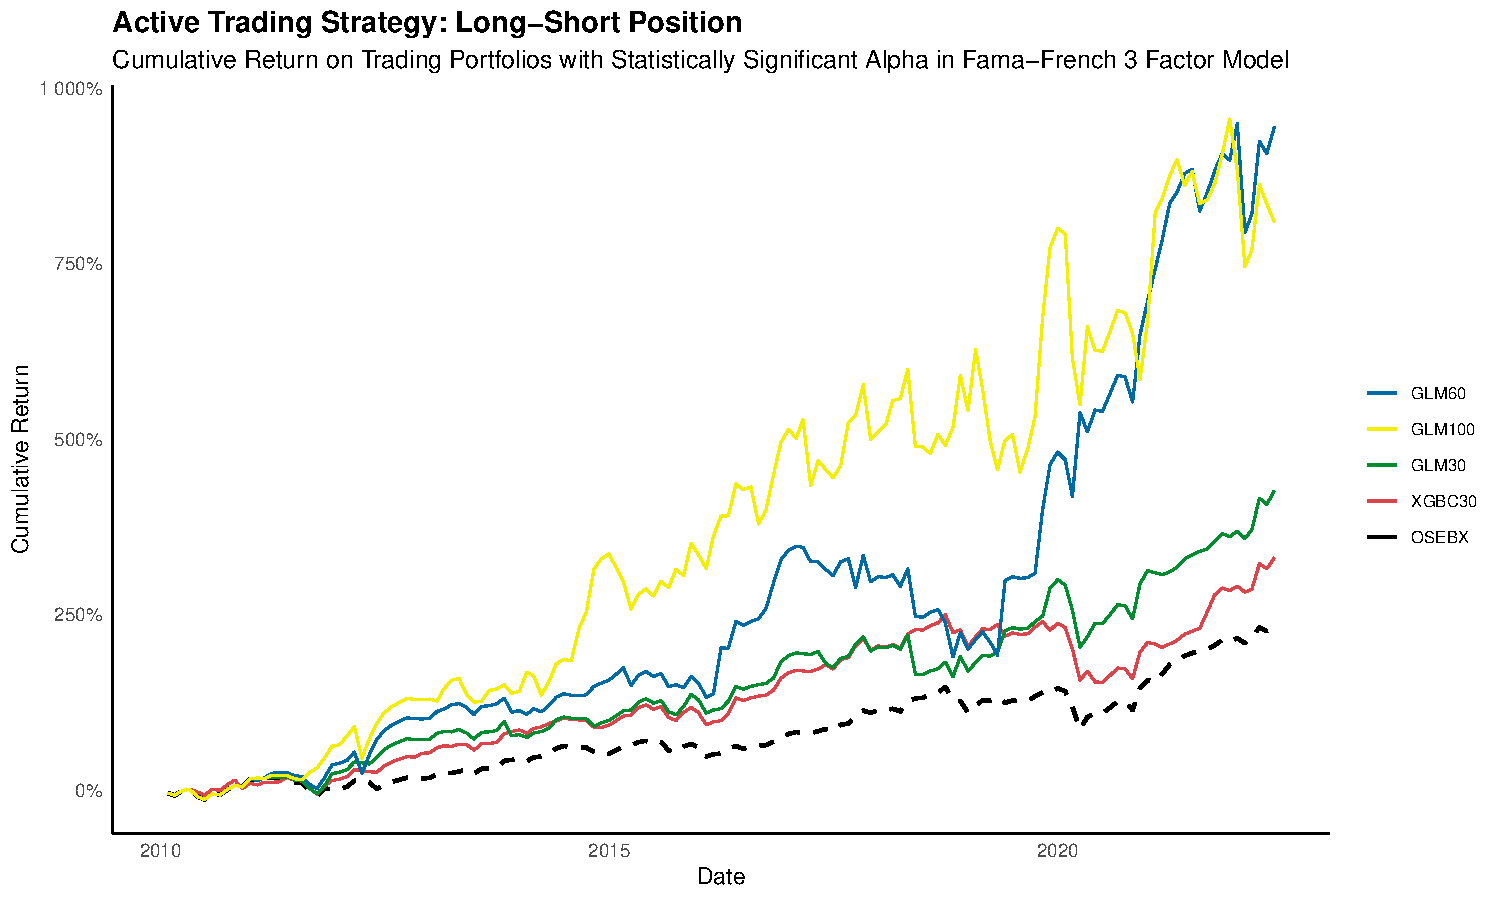
\includegraphics[width=0.85\textwidth]{images/trading_long_short.pdf}
    \caption{{Cumulative Return Long-Short Active Trading Strategy}}
    \subcaption*{Cumulative return for GLM30, GLM60, GLM100 and XGBC30, which all shows a significant alpha in the FF3-regression. OSEBX is also displayed. The GLM60 and GLM100 portfolios provide great investment opportunity for the risk-seeking investor.}
    \label{fig:long-short-top-5}
\end{figure}

\begin{figure}[H]
    \centering
    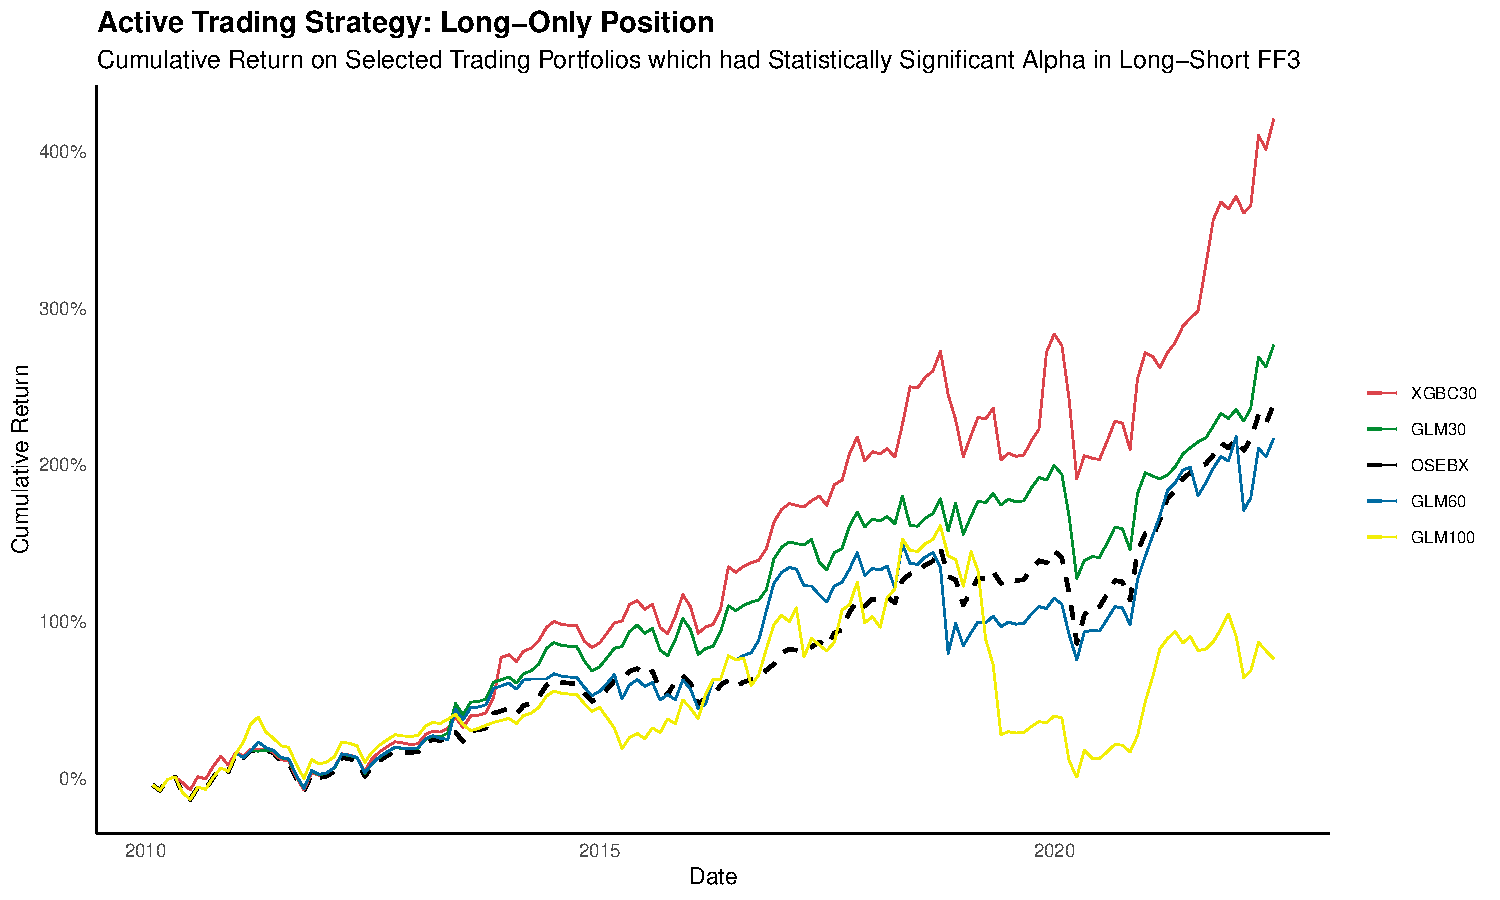
\includegraphics[width=0.85\textwidth]{images/trading_long_only.pdf}
    \caption{{Cumulative Return Long-Only Active Trading Strategy}}
    \subcaption*{Cumulative return for GLM30, GLM60, GLM100 and XGBC30, which all shows a significant alpha in the FF3-regression. OSEBX is also displayed. Still great returns for XGBC30 and GLM30, not so much for GLM60 and GLM100.}
    \label{fig:long-only-top-5}
\end{figure}

The cumulative return illustrated in \autoref{fig:long-short-top-5} shows that the GLM60 and GLM100 portfolios are yielding exceptional returns, though severely volatile. Those two portfolios are significantly affected by the low number of shares held in the active trading period, which varies between 1 and 6 companies. In contrast, the XGBC30 portfolio consist of about five times more, and still made for a significant alpha in the FF3-regression. Considering the long-only portfolios in \autoref{fig:long-only-top-5}, a different pattern emerges, where XGBC30L yields the highest returns, and the GLM60L and GLM100L perform worse than OSEBX when considering cumulative return. The predictions made by model XGBC30 seem to perform well in both strategies, and the increased number of shares seems to lower the risk in practice.

\subsubsection{Conclusion for Research Question (2)}
In this section, we have presented and discussed the results, to answer the research question: ”To what degree can trading on predicted additions and deletions outperform OSEBX in an active trading portfolio?". In this research question, we find that two types of very different portfolios tend to perform well. (1) The GLM portfolios predict few changes, but obtain excellent return on the few trades they do. (2) The XGBC30 portfolio can also obtain excellent returns but with a level of risk matching the benchmark, by predicting more changes than the GLM portfolios. Both directions tend to outperform OSEBX and have shown significant alphas in FF3. This is a \textit{key insight} in exploiting the index effect. Based on the results, it becomes evident that trading on predicted additions and deletions has proven to outperform OSEBX for the last 13 years, and we conclude that this strategy can outperform OSEBX to a high degree.  




% RESEARCH QUESTION 3 %%%%%%%%%%%%%%%%%%%%%%%%%%%%%%%%%%%%%%%%%%%%%%%%%%%

\subsection{Research Question (3): To what degree can trading on predicted additions and deletions outperform OSEBX in an enhanced index portfolio?}

In the previous two sections, we assessed the ML model performance of GLM and XGBoost and also applied them in an active trading strategy. Now we want to go further and investigate if such an active trading strategy can be combined with passive index investing to create an enhanced index portfolio, outperforming OSEBX.

\subsubsection{Enhanced Index Strategy}\label{Enhanced}

The enhanced index strategy seeks to combine the active trading strategy with an otherwise passive index portfolio. As discussed in \autoref{introduction}, defining enhanced index can be difficult \parencite{riepe-werner-are-enhanced-index-mutual-funds-worthy-of-their-name}. \textcite{ssg-tracking-error-enhanced} report that index investing can be considered "enhanced" with a TE in the continuum from 0.5\% to 2\%. We have decided to use a TE$_{ann}$ of 2\%, which is in the upper range of enhanced index. This enables us to more easily compare portfolio performances (as performance differences will grow with active share and TE). 

In practice, we adjust some of the financial assumptions, and run the simulations again, and use those to combine with OSEBX to construct enhanced index portfolios. We illustrate the enhanced index strategy in \autoref{fig:timeline-enhanced-index-investment-horizon}. Compared to the active trading strategy in \autoref{fig:timeline-investment-horizon}, we see that the active share is smaller, and the portfolio as a whole can therefore move closer to the benchmark index OSEBX. Note that we still use OSEBX as a benchmark index, which we calculate TE against, while we use OSEAX as the market in financial models.

\begin{figure}[H]
    \centering
    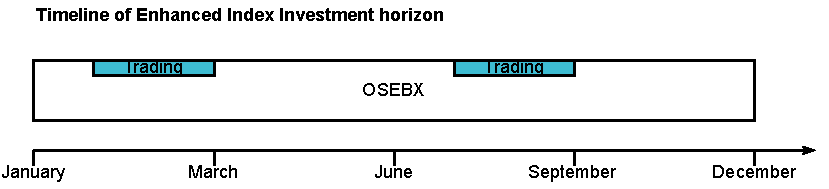
\includegraphics[width=\linewidth]{images/enhanced-index-investment-horizon.drawio.pdf}
    \vspace{1em}
    \caption{{Timeline of Enhanced Index Investment horizon}}
    \subcaption*{In the enhanced index portfolios, the active trading constitutes only for a smaller part of the total portfolio, which is dominated by OSEBX. }\vspace{1em}
    \label{fig:timeline-enhanced-index-investment-horizon}
\end{figure}

The simulated enhanced index funds consist of two parts. (1) The active share, which is a portfolio similar to those analysed in the previous section, and (2) The passive share, which is invested in OSEBX at all times. In contrast to the active trading perspective discussed in the previous section, we are now forced to own both the passive and the active share at the same time. The return of the enhanced index portfolios can be expressed as shown in \autoref{return_combined_port}, where $r_E$ is the return on the enhanced index portfolio, $r_A$ is the return on the active share, $r_P$ is the return of the passive share, and $s$ describes how big the active share is in the enhanced index portfolio. 

\begin{equation}
\begin{aligned}
    r_E =  r_A*s + r_P * (1-s)
\label{return_combined_port}
\end{aligned}
\end{equation}

\subsubsection{Financial Assumptions}

From the perspective of enhanced index portfolios, we face different challenges than those from the active trading portfolios. In this section, we are going to explore the most significant assumptions regarding the enhanced index portfolio, which can be broken down into interest rate on short positions, and share of active management.

We assume that by using an enhanced index strategy, we are managing a larger enhanced index fund, that follows OSEBX closely. By making this assumption, we always own stocks on OSEBX before each active investment horizon. This changes the assumption regarding short-position interest rates. Most importantly, we do not have to pay interest rates on the short positions. We would simply sell the positions because we already own them in the passive portfolio. Therefore, we simulate the active portfolios again, but this time without using interest rates on any short positions. 

Second, we assume that we are not allowed to operate outside the annual TE of 2\%. This limits how big a share of active management we can allow for throughout the year. How large the active management can be will depend on the prediction horizon of 30, 60, or 100 days, and also the volatility of the active portfolio. In this thesis, we have maximised the active share, given that TE cannot exceed 2\% annually. The weighting of the active share is therefore significantly varied between the portfolios. In general, the active portfolios with higher volatility are paired with a lower active share in the enhanced index portfolios. The weightings are shown in table \autoref{weights}. 

Third, the assumptions made in the previous section also apply in the context of an enhanced index portfolio, namely the assumptions regarding transaction costs, liquidity, and active portfolio weights (equal weighting of the companies held in the active part of the portfolio).

\subsubsection{Application of the Enhanced Portfolio Simulations}

The practical implementation of our enhanced index portfolio simulation closely mirrors that of the active trading portfolio simulation, but the main difference is that the enhanced portfolio is a combination of the active and the passive share. In practice, we first run new simulations of the active portfolios, without interest rates on short positions. Next, we optimise each active share, to yield a TE of 2\%. Finally, we analyse the performance of the enhanced index portfolios which are put together by combining the passive and active share using the weighting presented in \autoref{weights}.

\begin{table}[H]
\footnotesize
\center
\begin{tabular}{llll}
\toprule
Enhanced Portfolio & Active Share & Passive Share & TE_{ann} \\ 
\midrule
GLM30L & 0.267 & 0.733 & 2\% \\ 
XGBC30 & 0.221 & 0.779 & 2\%\\ 
XGBC30L & 0.182 & 0.818 & 2\%\\ 
GLM60L & 0.170 & 0.830 & 2\%\\ 
XGBB30 & 0.166 & 0.834 & 2\%\\ 
XGBB30L & 0.166 & 0.834 & 2\%\\ 
XGBC60L & 0.159 & 0.841 & 2\%\\ 
XGBC60 & 0.141 & 0.859 & 2\%\\ 
XGBB60L & 0.126 & 0.874 & 2\%\\ 
GLM100L & 0.124 & 0.876 & 2\%\\ 
GLM30 & 0.123 & 0.877 & 2\% \\ 
XGBC100 & 0.112 & 0.888 & 2\% \\ 
XGBB100 & 0.110 & 0.890 & 2\% \\ 
XGBC100L & 0.098 & 0.902 & 2\% \\ 
XGBB60 & 0.080 & 0.920 & 2\% \\ 
XGBB100L & 0.066 & 0.934 & 2\% \\ 
GLM60 & 0.041 & 0.959 & 2\% \\ 
GLM100 & 0.028 & 0.972 & 2\% \\ 
\bottomrule
\end{tabular}
\vspace{1em}
\caption{{Active and Passive Share in Enhanced Index Portfolios}}
\subcaption*{All portfolios are constructed to maximise the active share, and the constraint of TE cannot exceed 2\% per year. The active share represents the simulated portfolio trading on predicted additions/deletions, and the passive share is OSEBX.}
\label{weights}
\end{table}

In \autoref{weights}, we present the maximum weightings of the active share which is allowed in the enhanced index portfolios. This results in some interesting observations. First, we observe that the two most extreme active portfolios from the previous section (namely GLM60 and GLM100) are only allowed to constitute 4.1\% and 2.8\% as the active shares respectively. Secondly, the low-risk active portfolios like GLM30L (26.7\%), XGBC30 (22.1\%), and XGBC30L (18.2\%) are allowed to constitute an active share of several times more than the extreme portfolios.

\subsubsection{Performance in the Capital Asset Pricing Model}

Next, we investigate enhanced index portfolio performance. \autoref{tab:CAPM-PERFORMANCE-ENHANCED-INDEX} illustrate performance for the portfolios, sorted by decreasing SR. Notice that the name of the portfolio in \autoref{tab:CAPM-PERFORMANCE-ENHANCED-INDEX} corresponds to the active portfolio from \autoref{tab:machine-learning-model-names} used as the active share (without interest rate on short positions). 

% CAPM RESULTS
\begin{table}[H]
\centering
\footnotesize
\begin{tabularx}{\textwidth}{Xllllllll}
\toprule
Portfolio & $R_p-R_b$ & $R_p$ & $\sigma_p$    & SR & $\alpha$_{CAPM}  & $\beta$  & TE_{ann} & IR \\
\midrule
OSEBX &  0 & 0.0095 & 0.0423 & 0.1981 & 0.0002 & 1.0148 & 0.0000 &  \\ 
\midrule
GLM60 &  0.0005  & 0.0100 & 0.0410 & 0.2180 & 0.0011 & 0.9735 & 0.0200 & 0.0971 \\ 
GLM30 &  0.0005  & 0.0100 & 0.0418 & 0.2117 & 0.0008 & 0.9915 & 0.0200 & 0.0802 \\ 
GLM100 &  0.0003  & 0.0098 & 0.0412 & 0.2112 & 0.0008 & 0.9812 & 0.0200 & 0.0572 \\ 
XGBC30 &  0.0004  & 0.0099 & 0.0416 & 0.2111 & 0.0008 & 0.9933 & 0.0200 & 0.0721 \\ 
XGBB30 &  0.0001  & 0.0096 & 0.0420 & 0.2026 & 0.0004 & 1.0046 & 0.0200 & 0.0225 \\ 
XGBC100 &  -0.0005  & 0.0090 & 0.0392 & 0.2024 & 0.0003 & 0.9378 & 0.0200 & -0.0771 \\ 
XGBB60 &  -0.0003  & 0.0092 & 0.0407 & 0.2001 & 0.0003 & 0.9702 & 0.0200 & -0.0413 \\ 
XGBC60 &  -0.0004  & 0.0091 & 0.0407 & 0.1958 & 0.0001 & 0.9715 & 0.0200 & -0.0693 \\ 
XGBB100 &  -0.0006  & 0.0089 & 0.0399 & 0.1958 & 0.0001 & 0.9545 & 0.0200 & -0.0970 \\
\midrule
XGBC30L &  0.0006  & 0.0101 & 0.0423 & 0.2129 & 0.0008 & 1.0144 & 0.0200 & 0.1105 \\ 
XGBB30L &  0.0006  & 0.0101 & 0.0425 & 0.2112 & 0.0007 & 1.0217 & 0.0200 & 0.1033 \\ 
GLM30L &  0.0002  & 0.0097 & 0.0425 & 0.2021 & 0.0004 & 1.0083 & 0.0200 & 0.0359 \\ 
XGBC100L &  0.0000  & 0.0095 & 0.0414 & 0.2015 & 0.0003 & 0.9908 & 0.0200 & -0.0057 \\ 
XGBB60L &  0.0000  & 0.0095 & 0.0420 & 0.2008 & 0.0003 & 1.0044 & 0.0200 & 0.0104 \\ 
XGBB100L &  0.0000  & 0.0095 & 0.0420 & 0.1995 & 0.0002 & 1.0034 & 0.0200 & -0.0006 \\ 
XGBC60L &  0.0000  & 0.0095 & 0.0423 & 0.1982 & 0.0002 & 1.0092 & 0.0200 & 0.0004 \\ 
GLM60L &  -0.0001  & 0.0094 & 0.0429 & 0.1942 & 0.0001 & 1.0190 & 0.0200 & -0.0087 \\ 
GLM100L &  -0.0004  & 0.0091 & 0.0426 & 0.1872 & -0.0003 & 1.0180 & 0.0200 & -0.0705 \\ 
\bottomrule
\end{tabularx}
\vspace{1em}
\caption{{CAPM Portfolio Performance for Enhanced Index Strategies using Monthly Returns}}
\subcaption*{Risk free interest rate is $\approx$ 0.12 \% per month. The market return is assumed to be the return of OSEAX during the same period, which gave a monthly average return of $\approx$ 0.92\%. Both risk free interest rate and market return is calculated based on (\cite{bernt-fama-french}) in the period from January 31st 2010 to May 31st 2022. The TE and information ratio is calculated in relation to OSEBX, as this is the index we are aiming to beat. The table is sorted after SR. The analysed period is from January 31st 2010 to May 31st 2022. }
\label{tab:CAPM-PERFORMANCE-ENHANCED-INDEX}
\end{table}

Looking at \autoref{tab:CAPM-PERFORMANCE-ENHANCED-INDEX}, we find that GLM portfolios once again yield high SR, closely followed by XGBC30, XGBC30L, and XGBB30L. Also, when looking at the alpha $\alpha_{CAPM}$, GLM60 yields the highest, followed by GLM30, GLM100, XGBC30 and XGBC30L. In the enhanced portfolio simulation, the XGBC30L portfolio outperforms OSEBX the most, which seems to be a result of it being allowed to constitute for a significantly larger share (18.2\%) than the competing volatile portfolios. As we observed in the analysis of the active portfolios in the previous section, we see a tendency where the two styles of portfolios seem to outperform OSEBX. The first one is the high-yielding volatile portfolios, such as GLM60 and GLM100, and the second one is the diverse, low-risk portfolios.  

\subsubsection{Fama-French 3-factor Model}

In \autoref{fama-french-enhanced-long-short} and \autoref{fama-french-enhanced-long-only} we show FF3 regressions for long-short and long-only enhanced index portfolios respectively. 

% siste final allersiste oppdatert alt stemmer last and final update. Long short
\begin{table}[H] \centering 
\footnotesize
\begin{tabularx}{\textwidth}{XXXX|XXX|XXX|l} 
\\[-2ex]\hline 
\hline \\[-2ex] 
 & \multicolumn{10}{c}{\textit{Dependent variable:}} \\ 
\cline{2-11} 
\\[-2ex] 
 & \multicolumn{3}{c}{GLM} & \multicolumn{3}{c}{XGBB} & \multicolumn{3}{c}{XGBC} & \\
 \cline{2-10}
 \\[-2ex] 
 & 30 & 60 & 100 & 30 & 60 & 100 & 30 & 60 & 100 & OSEBX \\ 
 \cline{2-10} \\
 MR & 1.001$^{***}$ & 0.984$^{***}$ & 0.992$^{***}$ & 1.011$^{***}$ & 0.976$^{***}$ & 0.959$^{***}$ & 1.002$^{***}$ & 0.977$^{***}$ & 0.943$^{***}$ & 1.022$^{***}$ \\ 
  & (0.021) & (0.020) & (0.020) & (0.018) & (0.019) & (0.018) & (0.019) & (0.019) & (0.017) & (0.017) \\ 
   & & & & & & & & & & \\ 
 SMB & $-$0.060$^{***}$ & $-$0.046$^{**}$ & $-$0.047$^{**}$ & $-$0.054$^{***}$ & $-$0.047$^{**}$ & $-$0.027 & $-$0.064$^{***}$ & $-$0.046$^{**}$ & $-$0.027 & $-$0.042$^{**}$ \\ 
  & (0.021) & (0.020) & (0.020) & (0.018) & (0.019) & (0.018) & (0.019) & (0.019) & (0.017) & (0.017) \\ 
   & & & & & & & & & & \\ 
 HML & $-$0.020 & $-$0.029$^{*}$ & $-$0.031$^{**}$ & $-$0.007 & $-$0.005 & $-$0.008 & $-$0.013 & $-$0.007 & $-$0.010 & $-$0.016 \\ 
  & (0.015) & (0.015) & (0.015) & (0.013) & (0.014) & (0.013) & (0.014) & (0.014) & (0.013) & (0.013) \\ 
   & & & & & & & & & & \\ 
 $\alpha$_{FF3} & 0.001 & 0.001 & 0.001 & 0.001 & 0.001 & 0.0004 & 0.001$^{*}$ & 0.001 & 0.001 & 0.001 \\ 
  & (0.001) & (0.001) & (0.001) & (0.001) & (0.001) & (0.001) & (0.001) & (0.001) & (0.001) & (0.001) \\ 
   & & & & & & & & & & \\ 
\hline \\[-2ex] 
Obs & 148 & 148 & 148 & 148 & 148 & 148 & 148 & 148 & 148 & 148 \\ 
R$^{2}$ & 0.943 & 0.943 & 0.947 & 0.957 & 0.950 & 0.954 & 0.952 & 0.951 & 0.956 & 0.962 \\ 
R$^{2}$_{adj} & 0.942 & 0.942 & 0.946 & 0.956 & 0.949 & 0.953 & 0.951 & 0.950 & 0.955 & 0.961 \\ 

\hline 
\hline \\[-2ex] 
\textit{Note:}  & \multicolumn{10}{r}{$^{*}$p$<$0.1; $^{**}$p$<$0.05; $^{***}$p$<$0.01} \\ 
\end{tabularx} 
\vspace{1em}
\caption{{FF3 Regression: Long-Short Enhanced Index}} 
\subcaption*{The table shows the regression summary of the long-short enhanced portfolios return net of risk-free interest rate against market risk premium (RM), the small minus big factor (SMB), and the high minus low factor (HML). The market is considered to be OSEAX, the same we used in \autoref{tab:new-performance-trading-return-sigma-sharpe-alpha-beta-te-ir}. Notice that the factors are reported for OSE, and were obtained by \textcite{bernt-fama-french}}
\label{fama-french-enhanced-long-short} 
\end{table}

First of all, we notice that the coefficients have converged when comparing to the active trading FF3-regressions in \autoref{fama-french-trading-long-short} and \autoref{fama-french-trading-long-only}. This most likely comes from the fact that the enhanced index portfolios track OSEBX closely, and all portfolios are forced to track the index within the TE limit of 2\%. In other words, they will share risk and return characteristics with the benchmark. Interestingly, most of the coefficients to the risk factors are negative for enhanced index portfolios, similar to the same direction as the coefficients for the active portfolios \autoref{fama-french-trading-long-short}. A likely explanation for this is that OSEBX itself seems to be negatively correlated with the risk factors. Interestingly, most of the alphas for the long-short positions seem to be around 0.001. However, only the XGBC30 is significant (at a 90\% confidence level).

% siste final allersiste oppdatert alt stemmer last and final update. Long only
\begin{table}[H] \centering 
\footnotesize

\begin{tabularx}{\textwidth}{XXXX|XXX|XXX|l}
\\[-2ex]\hline 
\hline \\[-2ex] 
 & \multicolumn{10}{c}{\textit{Dependent variable:}} \\ 
\cline{2-11} 
\\[-2ex] 
 & \multicolumn{3}{c}{GLML} & \multicolumn{3}{c}{XGBBL} & \multicolumn{3}{c}{XGBCL} & \\
 \cline{2-10}
 \\[-1ex] 
 & 30 & 60 & 100 & 30 & 60 & 100 & 30 & 60 & 100 & OSEBX \\ 
 \cline{2-10} \\
 MR & 1.015$^{***}$ & 1.026$^{***}$ & 1.025$^{***}$ & 1.025$^{***}$ & 1.010$^{***}$ & 1.007$^{***}$ & 1.020$^{***}$ & 1.015$^{***}$ & 0.995$^{***}$ & 1.022$^{***}$ \\ 
  & (0.021) & (0.021) & (0.019) & (0.017) & (0.019) & (0.019) & (0.018) & (0.020) & (0.018) & (0.017) \\ 
   & & & & & & & & & & \\ 
 SMB & $-$0.051$^{**}$ & $-$0.030 & $-$0.026 & $-$0.032$^{*}$ & $-$0.028 & $-$0.017 & $-$0.035$^{*}$ & $-$0.030 & $-$0.019 & $-$0.042$^{**}$ \\ 
  & (0.022) & (0.021) & (0.019) & (0.017) & (0.019) & (0.019) & (0.018) & (0.020) & (0.018) & (0.017) \\ 
   & & & & & & & & & & \\ 
 HML & $-$0.010 & $-$0.021 & $-$0.021 & $-$0.003 & $-$0.013 & $-$0.011 & $-$0.010 & $-$0.016 & $-$0.013 & $-$0.016 \\ 
  & (0.016) & (0.016) & (0.014) & (0.012) & (0.014) & (0.014) & (0.013) & (0.014) & (0.014) & (0.013) \\ 
   & & & & & & & & & & \\ 
 $\alpha$_{FF3} & 0.001 & 0.0003 & $-$0.0001 & 0.001 & 0.001 & 0.0004 & 0.001 & 0.0004 & 0.0004 & 0.001 \\ 
  & (0.001) & (0.001) & (0.001) & (0.001) & (0.001) & (0.001) & (0.001) & (0.001) & (0.001) & (0.001) \\ 
   & & & & & & & & & & \\ 
\hline \\[-2ex] 
Obs & 148 & 148 & 148 & 148 & 148 & 148 & 148 & 148 & 148 & 148 \\ 
R$^{2}$ & 0.941 & 0.943 & 0.954 & 0.964 & 0.953 & 0.953 & 0.958 & 0.950 & 0.955 & 0.962 \\ 
R$^{2}$_{adj} & 0.940 & 0.942 & 0.953 & 0.963 & 0.952 & 0.952 & 0.957 & 0.949 & 0.954 & 0.961 \\ 

\hline 
\hline \\[-2ex] 
\textit{Note:}  & \multicolumn{10}{r}{$^{*}$p$<$0.1; $^{**}$p$<$0.05; $^{***}$p$<$0.01} \\ 
\end{tabularx} 
\vspace{1em}
\caption{{FF3 Regression: Long-Only Enhanced Index}} 
\subcaption*{The table shows the regression summary of the long-only enhanced portfolios return net of risk free interest rate against market risk premium (RM), the small minus big factor (SMB), and the high minus low factor (HML). The market is considered to be OSEAX, the same we used in \autoref{tab:new-performance-trading-return-sigma-sharpe-alpha-beta-te-ir}. Notice that the factors are reported for OSE, and were obtained by \textcite{bernt-fama-french}}
\label{fama-french-enhanced-long-only} 
\end{table} 

Furthermore, when considering the FF3 regressions for the enhanced long-only portfolios we get results quite similar to the enhanced long-short regressions, where the differences between the portfolios have converged. Also, we notice that none of the enhanced long-only portfolios are yielding significant alphas in the FF3-regressions. Even the strongest performing enhanced portfolio measured in $R_p$ XGBC30L is not significant, and neither are the other portfolios with high SR.

\subsubsection{Plot of Portfolios}

Next, we plot the portfolios with their cumulative return in comparison to the benchmark index OSEBX. The long-short and long-only enhanced index portfolios are shown in \autoref{fig:enhanced-long-short-top-5} and \autoref{fig:enhanced-long-only-top-5} respectively. The portfolios illustrated here are the same as we showed in the previous section (but now in enhanced portfolios). This is the GLM30, GLM60, GLM30, and XGBC30. Notice that all simulated enhanced portfolios are shown in \autoref{APPENDIX-Descriptive-statistics}, in \autoref{fig:enhanced-long-only-all} and \autoref{fig:enhanced-long-short-all}. 

\begin{figure}[H]
    \centering
    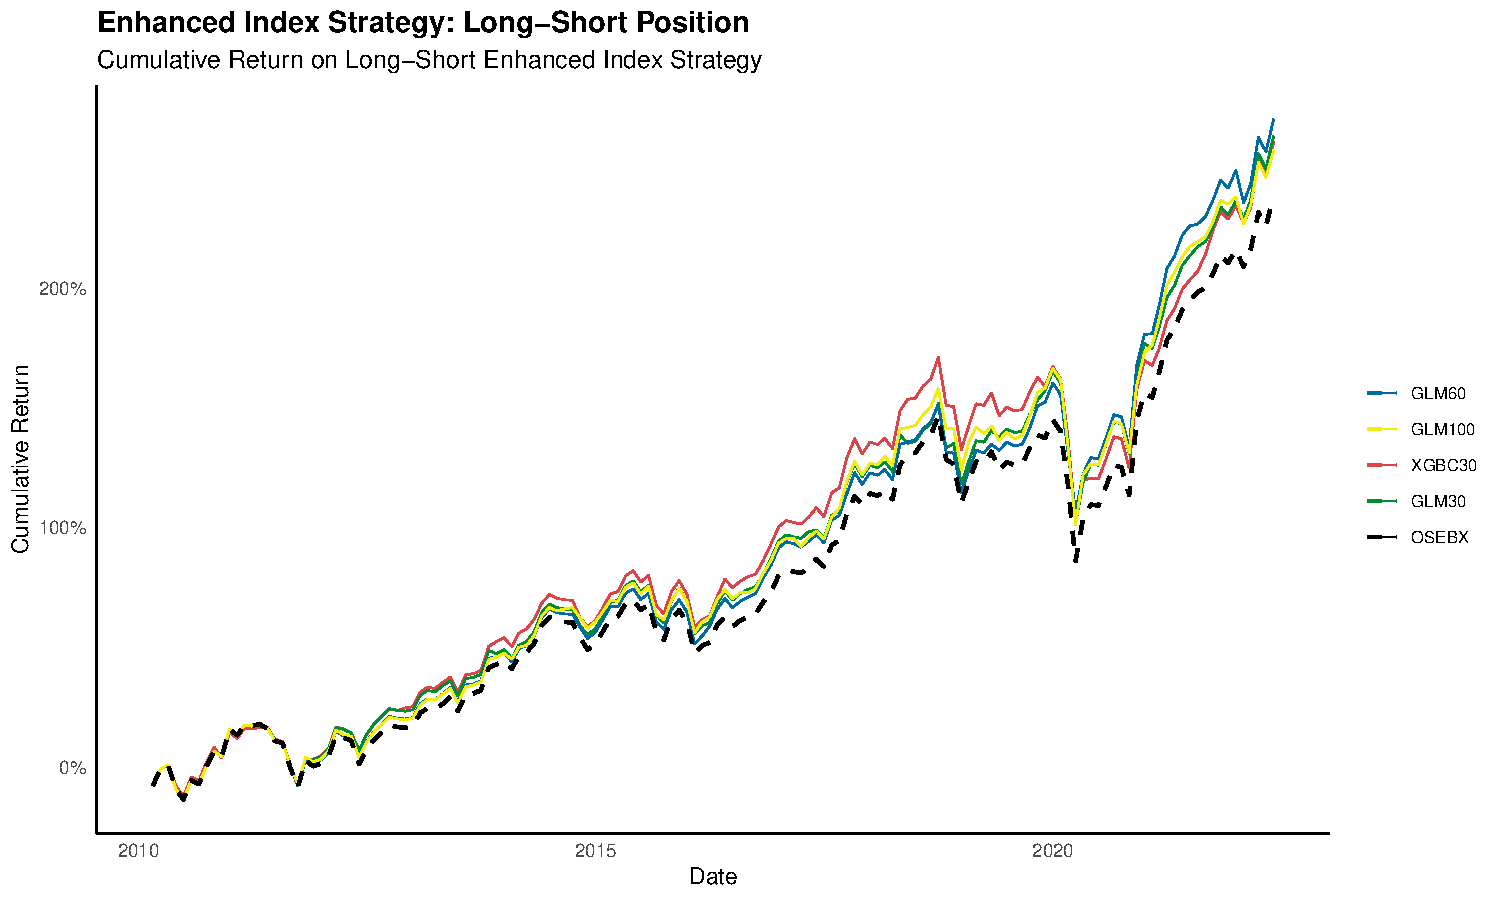
\includegraphics[width=0.9\textwidth]{images/enhanced_long_short.pdf}
    \caption{{Cumulative Return Long-Short Enhanced Index}}
    \subcaption*{Cumulative return for the enhanced long-short portfolios GLM30, GLM60, GLM100, XGBC30 and OSEBX. Only the XGBC30 portfolio yields a significant alpha in the FF3-regression.
    }
    \label{fig:enhanced-long-short-top-5}
\end{figure}

\begin{figure}[H]
    \centering
    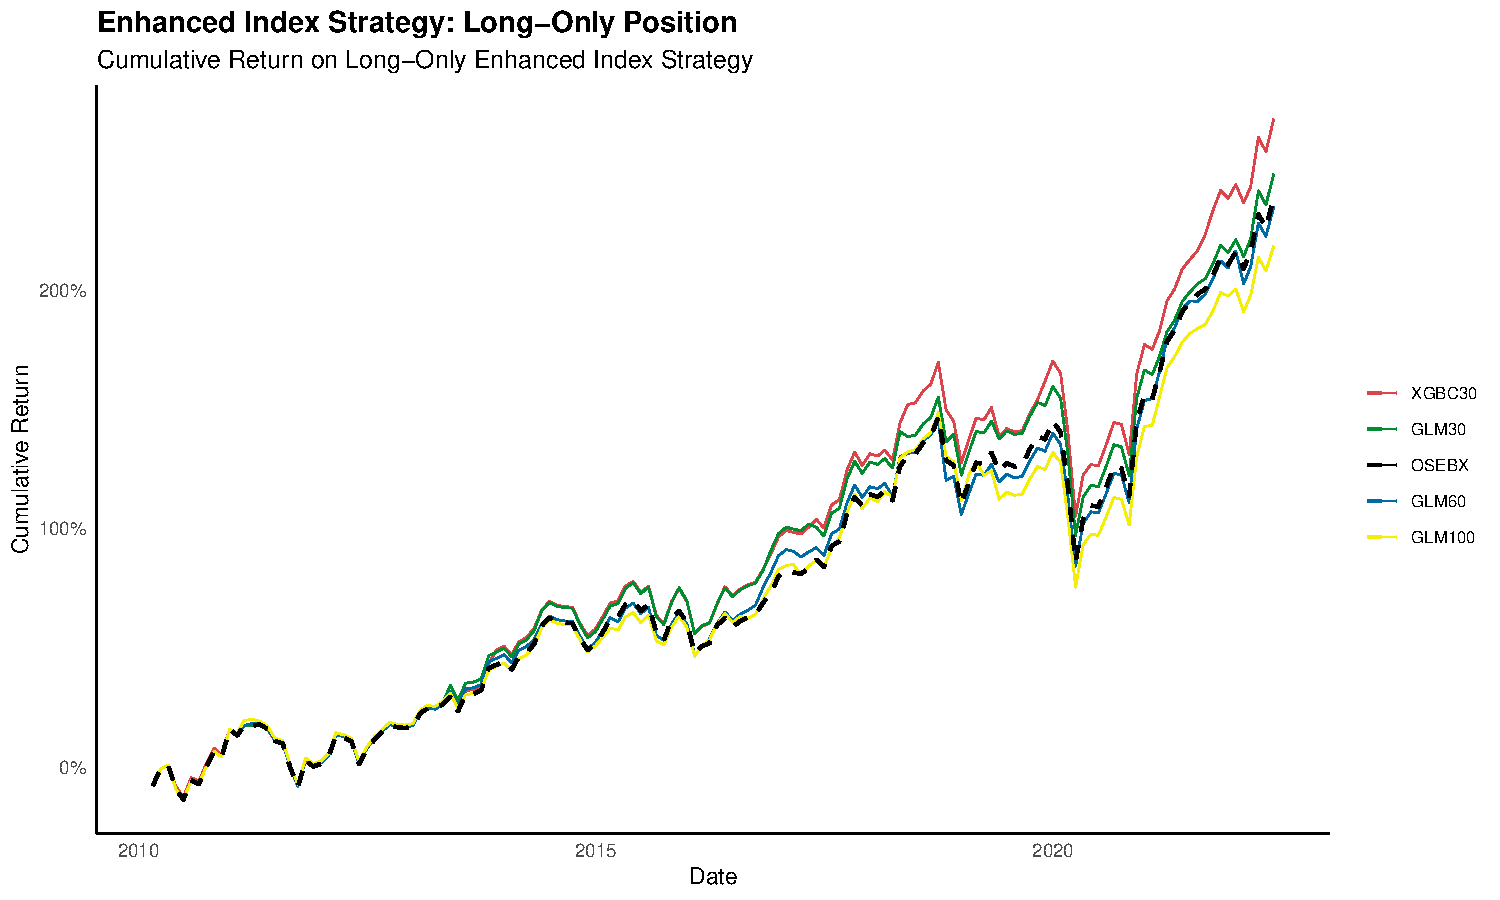
\includegraphics[width=0.9\textwidth]{images/enhanced_long_only.pdf}
    \caption{{Cumulative Return Long-Only Enhanced Index}}
    \subcaption*{Cumulative return for the enhanced long-only portfolios GLM30L, GLM60L, GLM100L, XGBC30L and OSEBX. None of the portfolios yielded significant alphas in the FF3-regression.}
    \label{fig:enhanced-long-only-top-5}
\end{figure}

When considering the visual representation of cumulative return for enhanced portfolios, once again a pattern emerges where the two portfolio types seem to perform well over time. In contrast to the active portfolios analysed in the previous section, the enhanced portfolios are seemingly less exposed to volatility, following OSEBX closely. 

\subsubsection{Conclusion for Research Question (3)}

Finally, our third research question was "To what degree can trading on predicted additions and deletions outperform OSEBX in an enhanced index portfolio?". In this section, we have analysed enhanced index portfolios, which were generated by combining the active trading portfolios from the previous section, with a passive share in OSEBX. The enhanced index portfolios were optimised to have a TE$_{ann}$ of 2\%. In \autoref{tab:CAPM-PERFORMANCE-ENHANCED-INDEX}, we found that several enhanced index portfolios yielded positive CAPM $\alpha_{CAPM}$ and outperformed OSEBX on metrics like $R_p$ and SR. But, in \autoref{fama-french-enhanced-long-short} and \autoref{fama-french-enhanced-long-only}, only the XGBC30 enhanced index portfolio gave a significant FF3 $\alpha_{FF3}$ at a 10\% confidence level after adjusting for risk factors. As expected, when combining the somewhat extreme GLM60 and GLM100 active portfolios with a passive portfolio, we are forced to use a lower active share due to the TE limit of 2\%. In contrast, the risk-averse portfolios allow for a bigger active share, making XGBC30L the highest-yielding enhanced index portfolio. 

In the previous section, we found that one can exploit the index effect by trading on (1) a few accurate predictions, or (2) more changes with a level of risk matching OSEBX. In an enhanced index portfolio, we find that only the latter approach yields significant excess returns in FF3. This is a \textit{key insight} when exploiting the index effect in an enhanced index portfolio. This must come from the fact that GLM can only constitute an active share of 2.8\%$-$4.1\%, compared to XGBC30 at 22.1\%, in an enhanced index portfolio. Finally, we were able to create enhanced index portfolios outperforming OSEBX over the last 13 years, and we conclude that we were able to outperform OSEBX to a reasonable extend.


